\documentclass[journal]{IEEEtran}
\usepackage[a5paper, margin=10mm]{geometry}
%\usepackage{lmodern} % Ensure lmodern is loaded for pdflatex
\usepackage{tfrupee} % Include tfrupee package


\setlength{\headheight}{1cm} % Set the height of the header box
\setlength{\headsep}{0mm}     % Set the distance between the header box and the top of the text


%\usepackage[a5paper, top=10mm, bottom=10mm, left=10mm, right=10mm]{geometry}

%
\usepackage{gvv-book}
\usepackage{gvv}
\setlength{\intextsep}{10pt} % Space between text and floats

\makeindex

\begin{document}
\bibliographystyle{IEEEtran}
\onecolumn
\newpage
\title{'2012-CE-'40-52''}
\author{AI24BTECH11004-Bheri Sai Likith Reddy}
\maketitle
\section{SECTION-A}

\begin{enumerate}
       \item Group I contains parameters and Group II lists methods/instruments.
	       
        \begin{align*}
             \begin{tabular}{c c}
                \textbf{Group I} & \textbf{Group II}\\
                P. Streamflow velocity  &  1. Anemometer\\
                    Q. Evapo-transpiration rate & 2. Penman's method \\
                R. Infiltration rate& 3. Horton's method\\
                S. Wind velocity&4. Current meter
             \end{tabular}
             \end{align*}
             \begin{enumerate}
             \item P-1,Q-2,R-3,S-4
             \item P-4,Q-3,R-2,S-1
             \item P-4,Q-2,R-3,S-1
             \item P-1,Q-3,R-2,S-4
        	\end{enumerate}	
	\item Wheat crop requires $55 cm$ of water during $120$ days of base period. The total rainfall during this period is $100 mm$ . Assume the irrigation efficiency to be $60 \%$. The area (in ha) of the land which can be irrigated with a canal flow of $0.01m^3/s$ is 
               \begin{enumerate}
			        \begin{multicols}{4}  
		       \item $13.82$
		       \item $18.85$
		       \item $23.04$
		       \item $230.40$
                    \end{multicols}   
	       \end{enumerate}	
       \item A water sample has a pH of 9.25 . The concentration of hydroxyl ions in the water sample is
		\begin{enumerate}
			\item $10^{-9.25}$ moles/L
			\item $10^{-4.75} mmoles/L$
			\item $0.302mg/L$
			\item $3.020mg/L$
		\end{enumerate}
	\item  A town is required to treat $4.2 m^{3} / min$ of raw water for daily domestic supply. Flocculating particles are to be produced by chemical coagulation. A column analysis indicated that an overflow rate of $0.2 mm / s$ will produce satisfactory particle removal in a settling basin at a depth of $3.5 m$ . The required surface area (in $m^{2}$ ) for settling is
		\begin{enumerate}
			\item $210$
			\item $350$
			\item$1728$
	        \item $21000$
        	\end{enumerate}
	\item A pavement designer has arrived at a design traffic of $100$ million standard axles for a newly developing national highway as per $IRC:37$ guidelines using the following data: design life = $15$ years, commercial vehicle count before pavement construction $=4500$ vehicles/day, annual traffic growth rate $=8 \%$. The vehicle damage factor used in the calculation was
		\begin{enumerate}
		       \item $1.53$
		       \item $2.24$
		       \item $3.66$
		       \item $4.14$
        	\end{enumerate}	
	\item The following data are related to a horizontal curved portion of a two-lane highway: length of curve $=200 m$, radius of curve $=300 m$ and width of pavement $=7.5 m$. In order to provide a stopping sight distance (SSD) of $80$ m , the set back distance (in m ) required from the centre line of the inner lane of the pavement is
		\begin{enumerate}
			\item $2.54$
			\item $4.55$
			\item $7.10$ 
			\item $7.96$ 
        	\end{enumerate}
	\item A two-lane urban road with one-way traffic has a maximum capacity of $1800$ vehicles/hour. Under the jam condition, the average length occupied by the vehicles is $5.0$ m . The speed versus density relationship is linear. For a traffic volume of $1000$ vehicles/hour, the density (in vehicles/km) is
		\begin{enumerate}
		       \item $52$
		       \item $58$
		       \item $67$
		       \item $75$
        	\end{enumerate}	
	\item The horizontal distance between two stations $P$ and $Q$ is $100 m$ . The vertical angles from $P$ and $Q$ to the top of a vertical tower at T are $3^{\circ}$ and $5^{\circ}$ above horizontal, respectively. The vertical angles from $P$ and $Q$ to the base of the tower are $0.1^{\circ}$ and $0.5^{\circ}$ below horizontal, respectively. Stations $P$ , $Q$ and the tower are in the same vertical plane with $P$ and $Q$ being on the same side of $T$. Neglecting earth's curvature and atmospheric refraction, the height (in m ) of the tower is
		\begin{enumerate}
			\item $6.972$
            \item $12.387$
            \item $12.540$
            \item $128.745$
        	\end{enumerate}	
    \textbf{common data for questions 48 and 49:}
    The flow net around a sheet pile wall is shown in the sketch. The properties of the soil are: permeability coefficient $=0.09 m /$ day \brak{isotropic}, specific gravity $=2.70$ and void ratio $=0.85$. The sheet pile wall and the bottom of the soil are impermeable.

\begin{figure}[h!]
    \centering
    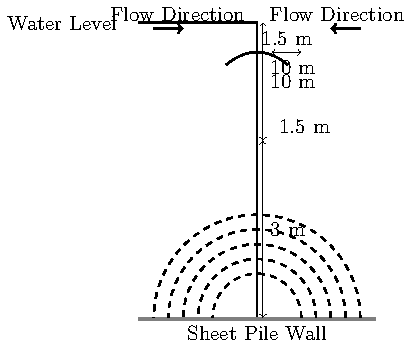
\includegraphics[width=0.7\textwidth]{fig/fig1.pdf}
\end{figure}
    
	\item  The seepage loss $\brak{\text{in } m^{3} \text{per day per unit length of the wall}}$ of water is
		\begin{enumerate}
            \begin{multicols}{4}
			\item $0.33$
			\item $ 0.38$
			\item $ 0.43$
			\item $ 0.54$
   \end{multicols}
        	\end{enumerate}	
	\item The factor of safety against the occurrence of piping failure is
                \begin{enumerate}
                \begin{multicols}{4}
			\item $3.55$
			\item $2.93$
			\item $ 2.60$
			\item $ 0.39$
        	\end{multicols}
         \end{enumerate}		
\textbf{Common data for questions 50 and 51:}
       An activated sludge system (sketched below) is operating at equilibrium with the following information. Wastewater related data: flow rate $=500 m^{3} /$ hour, influent $BOD=150 mg / L$, effluent BOD $=10 mg / L$. Aeration tank related data: hydraulic retention time $=8$ hours, mean-cell-residence time $=240$ hours, volume $=4000 m^{3}$, mixed liquor suspended solids 
       \begin{figure}[h!]
    \centering
    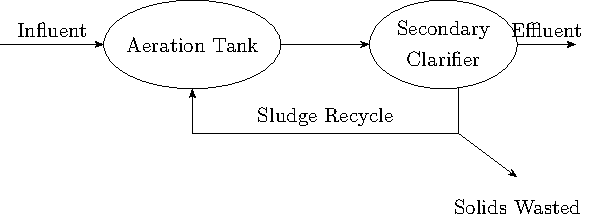
\includegraphics[width=0.7\textwidth]{fig/fig2.pdf}
\end{figure}
       
	\item  The food-to-biomass \brak{F/M} ratio $\brak{\text{in kg BOD per kg biomass per day}}$ for the aeration tank is
		\begin{enumerate}
			\item $0.015$
			\item $0.210$
			\item $0.225$
			\item $0.240$
        	\end{enumerate}	
	\item The mass \brak{\text{in kg/day}} of solids wasted from the system is
		\begin{enumerate}
			\item $58.9 s$
			\item $75 s$
			\item $100 s$
			\item $150 s$
        	\end{enumerate}	
\textbf{Linked Answer Questions}\\
\textbf{Statement for Linked Answer Questions 52 and 53:}
	The cross-section at mid-span of a beam at the edge of a slab is shown in the sketch. A portion of the slab is considered as the effective flange width for the beam. The grades of concrete and reinforcing steel are $M25$ and Fe $415$ , respectively. The total area of reinforcing bars $\brak{A_{s}}$ is $4000 mm^{2}$. At the ultimate limit state, $x_{u}$ denotes the depth of the neutral axis from the top fibre. Treat the section as under-reinforced and flanged $\brak{x_{u}>100 mm}$.

 \begin{figure}[h!]
    \centering
    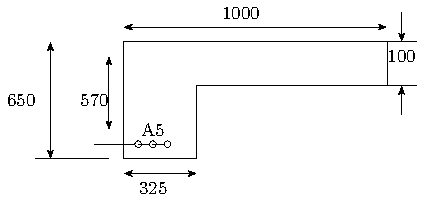
\includegraphics[width=0.7\textwidth]{fig/fig3.pdf}
\end{figure}
 all dimensions in $mm$
       \item The value of $x_{u}$ (in $mm$) computed as per the Limit State Method of IS $456:2000$ is
		\begin{enumerate}
			\item $200.0$
			\item $223.3$
			\item $236.3$
			\item $273.6$
        	\end{enumerate}	
\end{enumerate}	
\end{document}

